\documentclass[a4paper,11pt]{report}
\usepackage{geometry}
\geometry{margin=0.7in}
\usepackage{graphicx}
\usepackage{listings}
\usepackage{booktabs}
\usepackage{subcaption}

\begin{document}
\title{Labwork 4: CPU vs GPU Grayscale Conversion}
\author{Nguyen Phong Chau - 2540008}
\maketitle

\section*{Code}
\begin{lstlisting}[language=Python]
@cuda.jit
def grayscale_gpu_2d(src, dst) -> None:

    tidx = cuda.threadIdx.x + cuda.blockIdx.x * cuda.blockDim.x
    tidy = cuda.threadIdx.y + cuda.blockIdx.y * cuda.blockDim.y
    g = np.uint8(
        (src[tidx, tidy, 0] + src[tidx, tidy, 1] + src[tidx, tidy, 2]) / 3)
    dst[tidx, tidy, 0] = dst[tidx, tidy, 1] = dst[tidx, tidy, 2] = g
\end{lstlisting}

\section*{Mean time by block sizes between 1D and 2D}


\begin{table}[htbp]
\centering
\caption{Average CPU and GPU processing times by block size}
\begin{tabular}{rrrrr}
\toprule
Order & Dim & Threads & BlockSize & Time (ms) \\
\midrule
0 & 1D & 16 & 16 & 3.682668 \\
1 & 1D & 32 & 32 & 3.323858 \\
2 & 1D & 64 & 64 & 3.561551 \\
3 & 1D & 128 & 128 & 3.644618 \\
4 & 1D & 256 & 256 & 3.392350 \\
5 & 1D & 512 & 512 & 3.365658 \\
6 & 1D & 1024 & 1024 & 3.559546 \\
7 & 2D & 16 & 4:4 & 3.551440 \\
8 & 2D & 32 & 4:8 & 3.351309 \\
9 & 2D & 32 & 8:4 & 3.662337 \\
10 & 2D & 64 & 8:8 & 3.266118 \\
11 & 2D & 256 & 16:16 & 3.607598 \\
12 & 2D & 1024 & 32:32 & 4.407547 \\
\bottomrule
\end{tabular}
\end{table}

\section*{Original vs 1D vs 2D at block size 64}

\begin{figure}[htbp]
\centering
\begin{minipage}{0.32\textwidth}
    \centering
    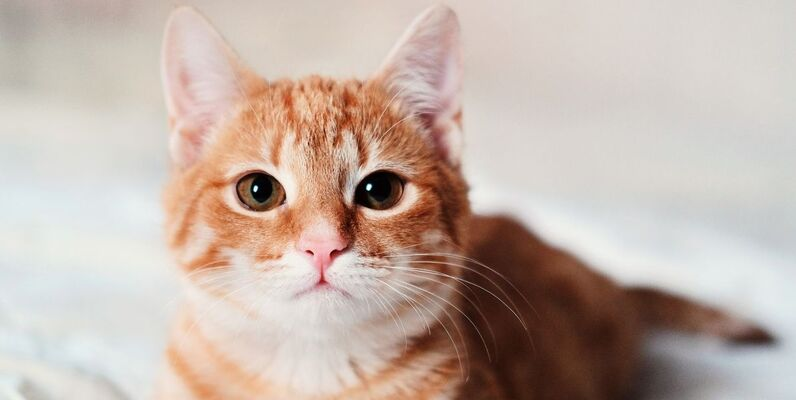
\includegraphics[width=\linewidth]{cat.jpg}
    \caption*{Original}
\end{minipage}
\hfill
\begin{minipage}{0.32\textwidth}
    \centering
    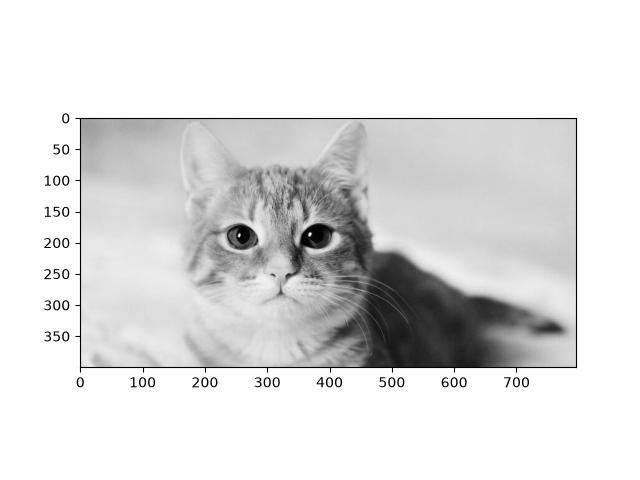
\includegraphics[width=\linewidth]{cat_1d_64.jpg}
    \caption*{1D GPU, 64}
\end{minipage}
\hfill
\begin{minipage}{0.32\textwidth}
    \centering
    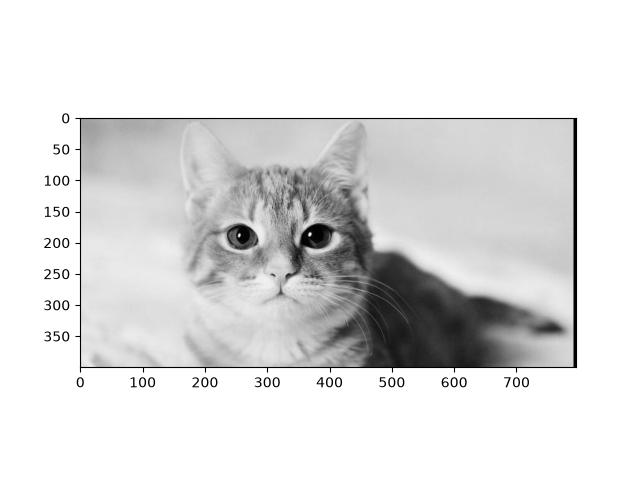
\includegraphics[width=\linewidth]{cat_2d_64.jpg}
    \caption*{2D GPU, 64}
\end{minipage}
\caption{Cat image comparison: original, 1D CUDA, and 2D CUDA results at block size 64.}
\end{figure}

\begin{figure}[htbp]
\centering
\begin{minipage}{0.32\textwidth}
    \centering
    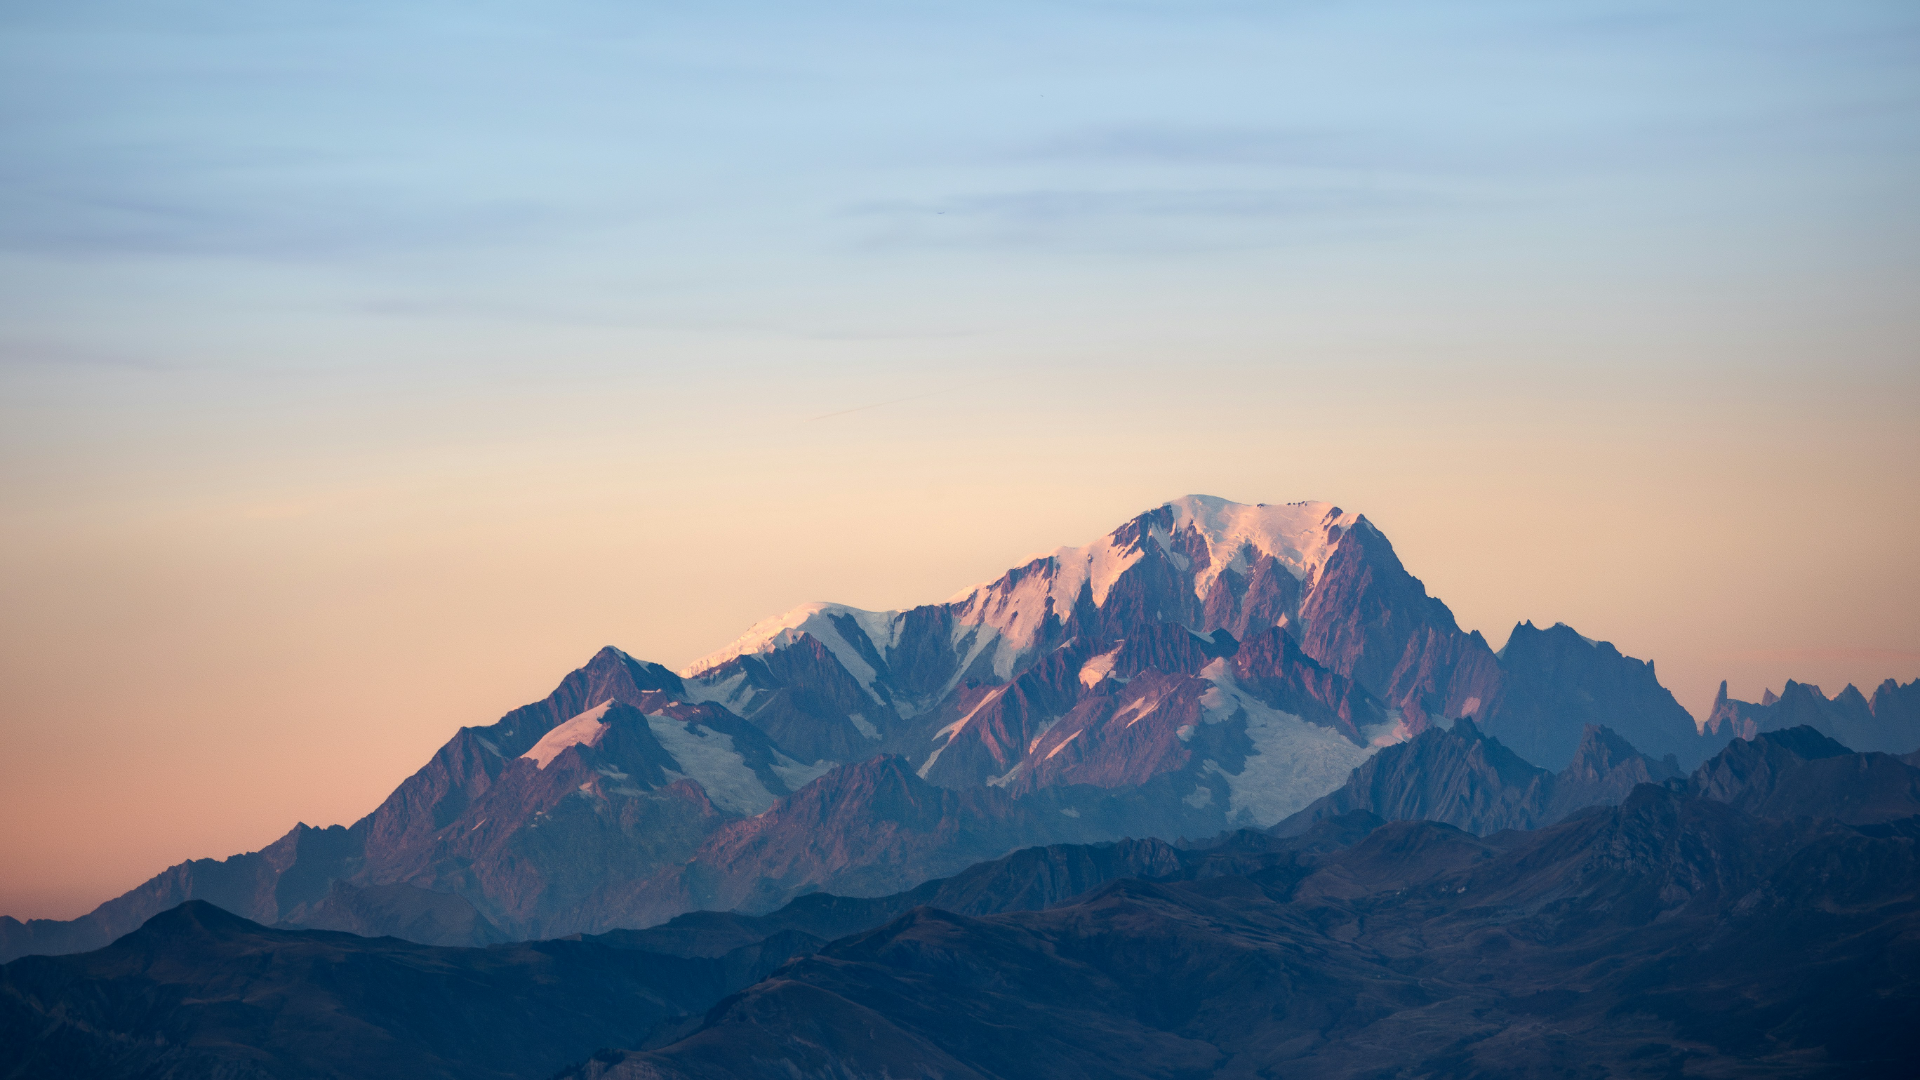
\includegraphics[width=\linewidth]{wallhaven.png}
    \caption*{Original}
\end{minipage}
\hfill
\begin{minipage}{0.32\textwidth}
    \centering
    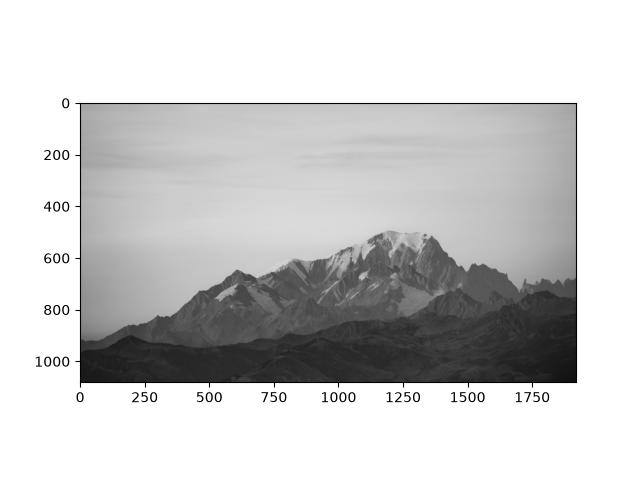
\includegraphics[width=\linewidth]{wall_1d_64.jpg}
    \caption*{1D GPU, 64}
\end{minipage}
\hfill
\begin{minipage}{0.32\textwidth}
    \centering
    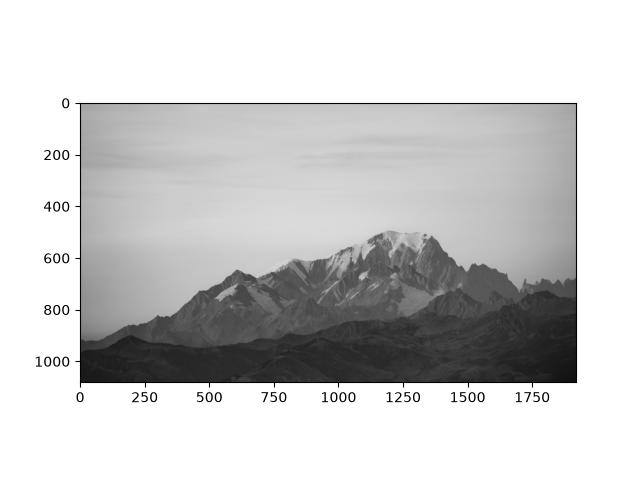
\includegraphics[width=\linewidth]{wall_2d_64.jpg}
    \caption*{2D GPU, 64}
\end{minipage}
\caption{Wall image comparison: original, 1D CUDA, and 2D CUDA results at block size 64.}
\end{figure}

\begin{figure}[ht]
        \centering
        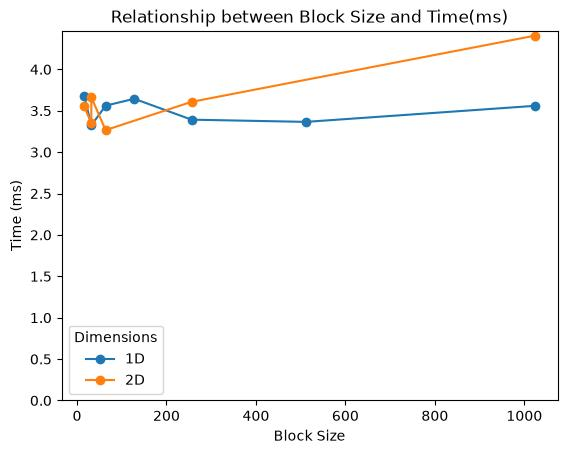
\includegraphics[width=0.8\textwidth]{relationship.jpg}
        \caption{Mean time by block size and block dimension.}
\end{figure}
\end{document}
